
\subsection{Soluzioni di esercizi nella sezione ``\textbf{\nameref{subsec:the:circle}}"}

% https://math.libretexts.org/Courses/Monroe_Community_College/MTH_165_College_Algebra_MTH_175_Precalculus/03%3A_Polynomial_and_Rational_Functions/3.02%3A_Circles/3.2e%3A_Circle_Exercises.
% https://math.libretexts.org/Courses/Monroe_Community_College/MTH_165_College_Algebra_MTH_175_Precalculus/03%3A_Polynomial_and_Rational_Functions/3.02%3A_Circles/3.2e%3A_Circle_Exercises.

Soluzione dell'esercizio \ref{circ_00} a pagina \pageref{circ_00}\label{circs_00}

\[
(x-8)^2+(y+10)^2=64
\]

\vspace{1cm}
\hrule
\vspace{1cm}


Soluzione dell'esercizio \ref{circ_01} a pagina \pageref{circ_01}\label{circs_01}

Center: $(2,1)$

Radius: $r=2$
\[
(x-2)^2+(y+1)^2=4
\]

\vspace{1cm}
\hrule
\vspace{1cm}


Soluzione dell'esercizio \ref{circ_02} a pagina \pageref{circ_02}\label{circs_02}

Center: $(-1,3)$

Radius:  $r=5$

\[
(x+1)^2+(y-3)^2=25  
\]

\vspace{1cm}
\hrule
\vspace{1cm}


Soluzione dell'esercizio \ref{circ_03} a pagina \pageref{circ_03}\label{circs_03}

\begin{itemize}
\item[a] Center $(2,-3)$, radius  $r=3$
\item[b] Center $(2,-5)$, radius  $r=2$
\item[c] Center $(-9,0)$, radius  $r=5$
\item[d] Center $(-\frac{1}{2},\frac{3}{5})$, radius  $r=\frac{\sqrt{161}}{10}$
\end{itemize}


\begin{figure}[H]
\centering
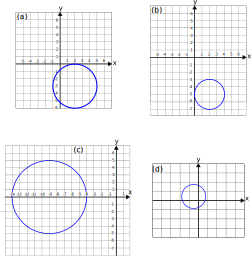
\includegraphics[width=0.9\textwidth]{circles_02.pdf}
\end{figure}




\vspace{1cm}
\hrule
\vspace{1cm}


Soluzione dell'esercizio \ref{circ_04} a pagina \pageref{circ_04}\label{circs_04}

\vspace{1cm}

Bisogna riscrivere l'equazione 

\[
x^2+y^2-6x+8y+24=0 
\]

nella forma dell'equazione standard del cerhio (l'equazione \ref{cerchio:equazione} a pagina \pageref{cerchio:equazione}):


\[
(x-h)^2+(y-k)^2=r^2
\]

Per fare ciò, spostiamo i termini variabili alla sinistra e le costanti a destra del segno di uguaglianza, e concentriamo l'attenzione sui termini con la $x$:

\begin{equation} \label{circ:04:1}
\underline{x^2-6x}+y^2+8y=-24
\end{equation}

Ora teniamo bene a mente come è fatto il quadrato del binomio:

\[
(x-h)^2 = x^2-2hx +h^2
\]

Guardando bene i termini con la $x$ nell'espressione \ref{circ:04:1}, troveremo che quel $-6x$ somiglia molto a $2\times -3\times x$, quindi basterebbe avere un $9$ per poter costruire un perfettamente plausibile quadrato: $x^2-6x+9$, il che ci direbbe che $h=-3$.

Possiamo aggiungere $9$ ad entrambi i termini dell'uguaglianza:


\[
\underline{x^2
-6x
+9
}
+y^2
+8y=-24 + 9 
\]

Ora possiamo raggruppare $x$:


\[
\underline{(x-3)^2 }
+y^2
+8y=-24 + 9 
\]

Facciamo lo stesso giochino con le $y$ , in quanto $+8y$ è $2\times 4 \times y$ quindi aggiungiamo $16$ da entrambe le parti come abbiamo fatto prima:

\[
(x-3)^2 
+y^2
+8y
+16
=-24 + 9 +16
\]

Ora l'equazione diventa:

\[
(x-3)^2+ 
(x+4)^2
=1
\]


Abbiamo quindi trovato i valori che ci serviuvano e cioè $h=3$, $k=-4$, $r=1$.

In altre parole il nostro cerchio ha il centro in $(3,-4)$ e un raggio pari a $1$.



\vspace{1cm}
\hrule
\vspace{1cm}


Soluzione dell'esercizio \ref{geop_01} a pagina \pageref{geop_01}\label{geos_01}

The tangent(s) are of the form $y = mx + 14$ because they go through $(0,14)$.

Substitute this into the equation of the circle:


\[
x^2+y^2+14x-6y=-41
\]

\[
x^2+(mx+14)^2+14x-6(mx+14)+41=0
\]


\[
x^2+m^2x^2+28mx+196+14x-6mx-43=0
\]

\[
(1+m^2)x^2+(22m+14)x+153=0
\]

This is a quadratic equation: $ax^2+bx+c=0$
where
\begin{enumerate}
\item $a=1+m^2$
\item $b=22m+14$
\item $c=153$
\end{enumerate}

The discriminant ($b^2-4ac$) tells us how many solutions does the equation have.

In this case we are looking for a single solution because the lines are tangent to the circle, i.e. each line touches the circle in one point only.

So the discriminant (often written as $\Delta$) must be zero:

\[
(22m+14)^2-4(1+m^2)153=0
\]

\[
484m^2+616m+196-612-612m^2=0
\]

\[
-128m^2+616m-416=0
\]

Now this is a simple quadratic equation, let's apply the formula:

\[
m=\frac{-b\pm\sqrt{b^2-4ac}}{2a}=\frac{-616\pm \sqrt{616^2-4\times(-128)\times(-416)}}{2\times -128}
\]


\[
m=\frac{-616\pm \sqrt{379456-212992}}{-256}
\]


\[
m=\frac{-616\pm 408}{-256}
\]

\[
\left\{
\begin{array}{ll}
m_1=\frac{-616+408}{-256}=\frac{-208}{-256}=\frac{13}{16}\\
\\
m_2=\frac{-616-408}{-256}=4
\end{array}
\right.
\]

\[
\left\{
\begin{array}{ll}
l_1: y=\frac{13}{16}x+14\\
\\
l_2: y=4x+14
\end{array}
\right.
\]

\vspace{1cm}
\hrule
\vspace{1cm}


Soluzione dell'esercizio \ref{circ_06} a pagina \pageref{circ_06}\label{circs_06}

È necessario per prima cosa riscrivere le equazioni nella seguente forma:

\[
(x-h)^2+(y-k)^=r^2
\]

dove 
\begin{itemize}
\item[\textbf{h}] è la coordinata $x$ del centro
\item[\textbf{k}] è la coordinata $y$ del centro
\item[\textbf{r}] è il raggio
\end{itemize}

Raccogliendo per $x$ e $y$ otteniamo: 

\[
\begin{split}
(a): (x^2-2x)+(y^2-4y)=4 \\
\\
(b): (x^2-4x)+(y^2-2y)=-4
\end{split}
\]

Facendo riferimento per ora alla sola equazione $(a)$, per trasformare
i termini $(x^2-2x)$ e $(y^2-4y)$ nella forma $(x-h)^2, (y-k)^2$ dobbiamo
seguire per ognuno dei termini questi passi:

\begin{enumerate}
\item considerare il coefficiente del termine di primo grado
\item dividere per $2$
\item calcolarne il quadrato
\item aggiungere il risultato da entrambi i lati dell'equazione
\end{enumerate}

Questo significa che per il termine $(x^2-2x)$ avremo:

\begin{enumerate}
\item il coefficiente del termine di primo grado è $2$
\item $2/2=1$
\item $1^2=1$
\item aggiungere questo risultato a entrambi i lati dell'equazione, che diventa:
\[
(a): (x^2-2x+1)+(y^2-4y)=4+1
\]
\end{enumerate}

Per il termine $(y^2-4y)$ avremo che:
\begin{enumerate}
\item il coefficiente del termine di primo grado è $4$
\item $4/2=2$
\item $2^2=4$
\item aggiungere il risultato a entrambi i lati dell'equazione, che diventa:
\[
(a): (x^2-2x+1)+(y^2-4y+4)=4+1+4
\]
\end{enumerate}

A questo punto possiamo riscrivere l'equazione come segue:

\[
(a) (x-1)^2+(y-2)^2=3^2
\]

Quindi la prima circonferenza avrà il centro in $(1, 2)$ e raggio 3.

Allo stesso modo la seconda equazione potrà essere riscritta come segue:
\[
(b) (x-2)^2+(y-1)^2=1
\]

Quindi la seconda circonferenza avrà il centro in $(2, 1)$ e raggio 1.

Un veloce grafico ci dirà che la soluzione esatta è la $B$:
le due circonferenze sono disgiunte e la seconda è interna alla prima.

\begin{figure}[H]
\centering
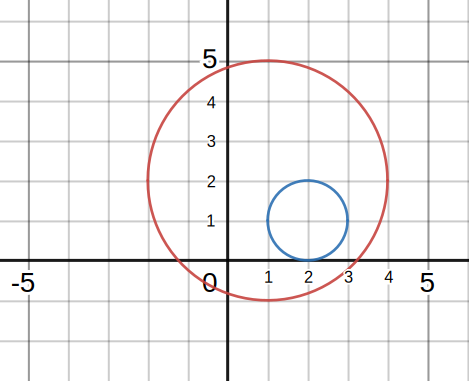
\includegraphics[width=0.6\textwidth]{circ_06.pdf}
\end{figure}

N.B.: la risposta $D$ era comunque da scartare in quanto due circonferenze
possono avere solo zero punti in comune (disgiunte) oppure un
punto in comune (tangenti) oppure due punti in comune (intersecanti),
oppure infiniti punti in comune (identiche e sovrapposte).



%\vspace{1cm}
%\hrule
%\vspace{1cm}
%
%
%Soluzione dell'esercizio \ref{circ_07} a pagina \pageref{circ_07}\label{circs_07}
%
%\vspace{1cm}
%\hrule
%\vspace{1cm}
%
%
%Soluzione dell'esercizio \ref{circ_08} a pagina \pageref{circ_08}\label{circs_08}
%
%\vspace{1cm}
%\hrule
%\vspace{1cm}
%
%
%Soluzione dell'esercizio \ref{circ_09} a pagina \pageref{circ_09}\label{circs_09}
%
%\vspace{1cm}
%\hrule
%\vspace{1cm}
%
%
%Soluzione dell'esercizio \ref{circ_10} a pagina \pageref{circ_10}\label{circs_10}
%
%\vspace{1cm}
%\hrule
%\vspace{1cm}
%


